\documentclass{article}
\usepackage{etex}
\usepackage{amsmath}
\usepackage{pdfpages}
\usepackage{tikz}
\usepackage{subcaption}
\usepackage{pgf-umlsd}
\usepackage{pgfplots}
\usepackage{geometry}
\usepackage{hyperref}
\geometry{
	a4paper,
	left=25.4mm,
	right=25.4mm,
	top=25mm,
	bottom=25.4mm
	}
\begin{document}

\includepdf{title.pdf}

\tableofcontents
\listoffigures

\newpage

\section{Statement of the problem}

Paxos solves Obstruction Free Consensus which has the following properties: 
\begin{itemize}
    \item \textbf{Obstruction Free Termination}: 1. If a correct process p proposes, it eventually decides or aborts.
    2. If a correct process decides, no correct process aborts infinitely often.
    3. If there is a time after which a single correct process p proposes a value sufficiently often, then p eventually decides.
    \item \textbf{Agreement}: No two processes decide differentely.
    \item \textbf{Validity}: Every decided value is a proposed value.
\end{itemize}

\section{Java Implementation of the Robust Key-Value Store}

\subsection{Java classes}
For our implementation with Java and the Akka framework, we have created the following classes:

\begin{itemize}
    \item \texttt{Main}: The main class that creates the different actors and configures the system. It is also the class that computes the statistics at the end of the simulation.

    \item \texttt{Process}: The actor class. The obstruction-free consensus algorithm is implemented in this class.

    \item \texttt{AbortMsg}: The class that represents the abort message sent between the processes.

    \item \texttt{AckMsg}: The class that represents the acknowledgment (ACK) message sent between the processes.

    \item \texttt{CrashMsg}: The class that represents the crash message sent between the processes. When a process receives a crash message, it will enter in the fault-prune mode.

    \item \texttt{DecideMsg}: The class that represents the decide message sent between the processes.

    \item \texttt{WriteAck}: The class that represents the write acknowledgments sent between the processes.

    \item \texttt{Pair}: Used to store (est and estballot) the values inside the states map.
    \item \texttt{GatherMsg}: The class that represents the GATHER message sent between the processes.
    
    \item \texttt{ImposeMsg}: The class that represents the IMPOSE message sent between the processes.
    
    \item \texttt{Members}: The class that contains the processes' references.
    
    \item \texttt{Pair}:  The class that represents a pair of values (est and estballot) used in the states map.
    
    \item \texttt{ReadMsg}: The class that represents the read message sent between the processes.
\end{itemize}

We didn't want to use multiple threads in the \texttt{Process} class due to the large number of processes
being launched. It is more efficient to let the Akka framework's logic thread handle the processes.
Therefore, we implemented a state machine in the \texttt{Process} class to manage the different states
of the functions: sending the initial read request, waiting for a quorum of responses, sending the
write request, and finally, waiting for a quorum of write acknowledgments.


\newpage
\subsection{Akka Sequence Diagram}

Let's consider an example of the case ($N=3$) in which only one process proposes and all 3 processes are correct processes.

\begin{figure}[h!]
\centering

\begin{sequencediagram}
    \newthread{main}{main}
    \newinst{a}{Correct Process  A}
    \newinst[1]{b}{Correct Process B}   
    \newinst[1]{c}{Correct Process C}

    \mess{main}{refs}{a}
    \mess{main}{refs}{b}
    \mess{main}{refs}{c}
    \mess{main}{launch}{a}
    \begin{sdblock}{Read Phase}{}
        \mess{a}{read}{a}
        \mess{a}{read}{b}
        \mess{a}{read}{c}
        \mess{c}{gather}{a}
        \mess{a}{gather}{a}
        \mess{main}{majority reached}{a}    
        \mess{b}{gather}{a}
        
    \end{sdblock}
    \begin{sdblock}{Impose Phase}{}
        \mess{a}{impose}{a}
        \mess{a}{impose}{b}
        \mess{a}{impose}{c}
        \mess{a}{ack}{a}
        \mess{c}{ack}{a}
        
        \mess{main}{ack majority reached}{a} 
        \mess{a}{decide}{b}
        \mess{a}{decide}{c}
        \mess{b}{ack}{a}
    \end{sdblock}
    
\end{sequencediagram}

\caption{Sequence diagram of the Akka design}
\end{figure}
\newpage
\subsection{Test machine configuration}
To compute the results, we used a laptop equipped with an AMD Ryzen 7 5800H processor, featuring 8 cores and 16 logical threads.

We also performed a warm-up round to minimize data aberrations caused by Java Virtual Machine (JVM) optimizations. However, we believe that some of our values may still be influenced by these optimizations.

The source code can be found here : \href{https://github.com/AdrienFL/Blockchain-Project}{https://github.com/AdrienFL/Blockchain-Project}

\newpage

\section{Performance analysis}
The simulation has different parameters that can be changed to test the performance of the system. The main parameters are:

\begin{itemize}
    \item $N$ The number of processes and $f$ the number of processes which can fail.
    \item $t_{le}$ The fixed timeout.
    \item $\alpha$ The probability of failure of a process.
\end{itemize}

Since we need a quorum, $f$ must be less than $N/2$. Thus,
we have different scenarios to test the performance of the simulation
with $(N,f) \in \{(3,1),(10,4),(100,49)\}$, $t_{le} \in \{0.5,1,1.5,2\}$ and $\alpha \in \{0,0.1,1\}$.

\subsection{Results for a fixed timeout $t_{le}$}
Let's now analyze the results for a fixed timeout $t_{le}$ and different values of $N$.

\begin{figure}[h!]
    \centering
    \begin{subfigure}{0.55\textwidth}
    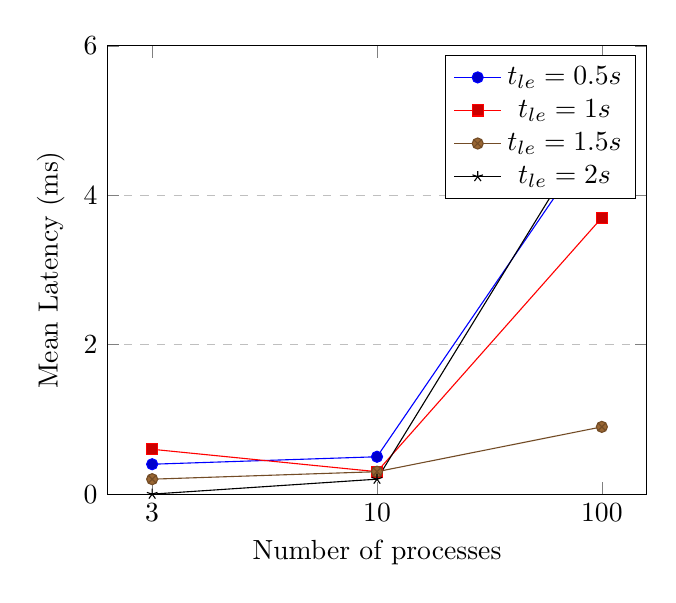
\begin{tikzpicture}
        \begin{axis}[
            xlabel={Number of processes},
            ylabel={Mean Latency (ms)},
            xtick=data,
            symbolic x coords={3, 10, 100},
            ymin=0, ymax=6,
            ymajorgrids=true,
            grid style=dashed
        ]
        \addplot coordinates {(3, 0.4) (10, 0.5) (100, 4.9)};
        \addlegendentry{$t_{le} = 0.5s$}
        \addplot coordinates {(3, 0.6) (10, 0.3) (100, 3.7)};
        \addlegendentry{$t_{le} = 1s$}
        \addplot coordinates {(3, 0.2) (10, 0.3) (100, 0.9)};
        \addlegendentry{$t_{le} = 1.5s$}
        \addplot coordinates {(3, 0.0) (10, 0.2) (100, 5.1)};
        \addlegendentry{$t_{le} = 2s$}
        \end{axis}
    \end{tikzpicture}
    \caption{Mean latency comparison for $\alpha = 0$}
\end{subfigure}%
\begin{subfigure}{.55\textwidth}
    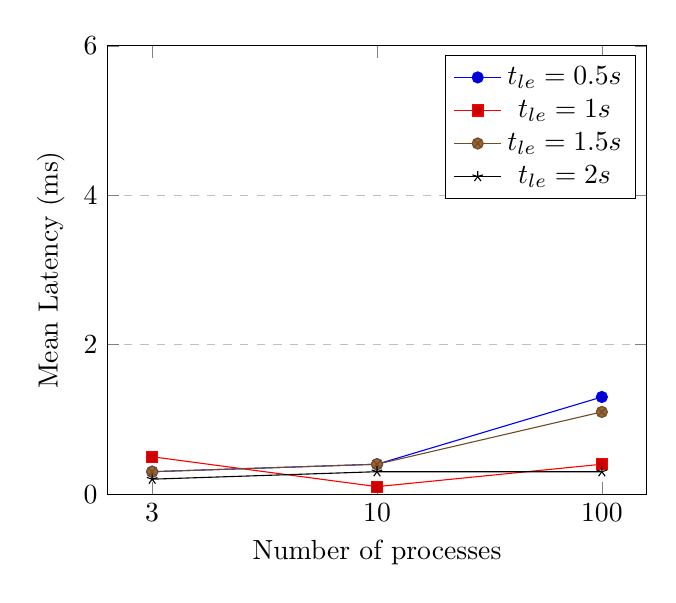
\begin{tikzpicture}
        \begin{axis}[
            xlabel={Number of processes},
            ylabel={Mean Latency (ms)},
            xtick=data,
            symbolic x coords={3, 10, 100},
            ymin=0, ymax=6,
            ymajorgrids=true,
            grid style=dashed
        ]
        \addplot coordinates {(3, 0.3) (10, 0.4) (100, 1.3)};
        \addlegendentry{$t_{le} = 0.5s$}
        \addplot coordinates {(3, 0.5) (10, 0.1) (100, 0.4)};
        \addlegendentry{$t_{le} = 1s$}
        \addplot coordinates {(3, 0.3) (10, 0.4) (100, 1.1)};
        \addlegendentry{$t_{le} = 1.5s$}
        \addplot coordinates {(3, 0.2) (10, 0.3) (100, 0.3)};
        \addlegendentry{$t_{le} = 2s$}
        \end{axis}
    \end{tikzpicture}
    \caption{Mean latency comparison for $\alpha = 0.1$}
\end{subfigure}
\begin{subfigure}{.55\textwidth}
    \vspace{1cm}
    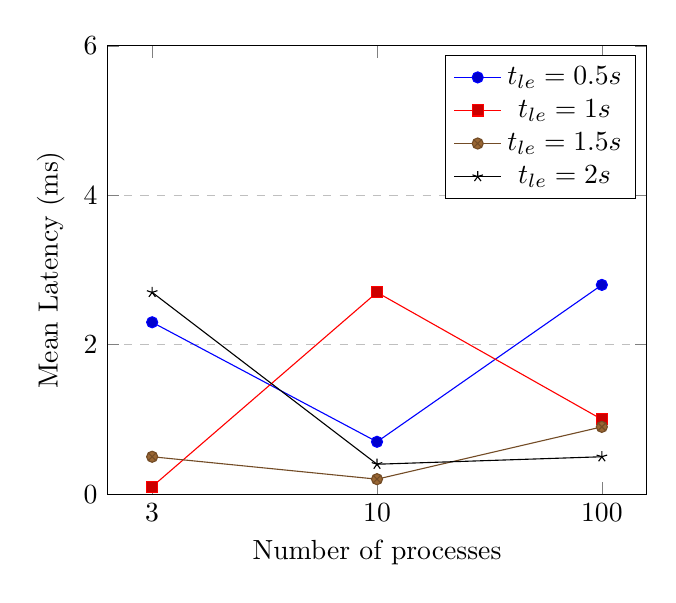
\begin{tikzpicture}
        \begin{axis}[
            xlabel={Number of processes},
            ylabel={Mean Latency (ms)},
            xtick=data,
            symbolic x coords={3, 10, 100},
            ymin=0, ymax=6,
            ymajorgrids=true,
            grid style=dashed
        ]
        \addplot coordinates {(3, 2.3) (10, 0.7) (100, 2.8)};
        \addlegendentry{$t_{le} = 0.5s$}
        \addplot coordinates {(3, 0.1) (10, 2.7) (100, 1.0)};
        \addlegendentry{$t_{le} = 1s$}
        \addplot coordinates {(3, 0.5) (10, 0.2) (100, 0.9)};
        \addlegendentry{$t_{le} = 1.5s$}
        \addplot coordinates {(3, 2.7) (10, 0.4) (100, 0.5)};
        \addlegendentry{$t_{le} = 2s$}
        \end{axis}
    \end{tikzpicture}
    \caption{Mean latency comparison for $\alpha = 1$}
\end{subfigure}
\caption{Mean latency comparison for fixed timeout and alpha values and different number of processes}
\end{figure}
Since consensus is reached before the call to \textit{hold}, the differences in the \( t_{le} \) values do not significantly impact performance. In a larger system, having a timeout is very useful, because it allows the system to still be able to reach a consensus by reducing the number of proposing process to only one.
The choice of timeout should balance failure detection and system stability. A timeout that is too long delays the election of a new leader when a failure occurs, increasing recovery time. On the other hand, a well-chosen timeout ensures that the system remains responsive without unnecessary leader use.

\newpage

\subsection{Results for a fixed number of processes}
Let's first analyze the results for a fixed number of processes $N$ and different values of $t_{le}$.

\begin{figure}[h!]
    \centering
    \begin{subfigure}{0.55\textwidth}
    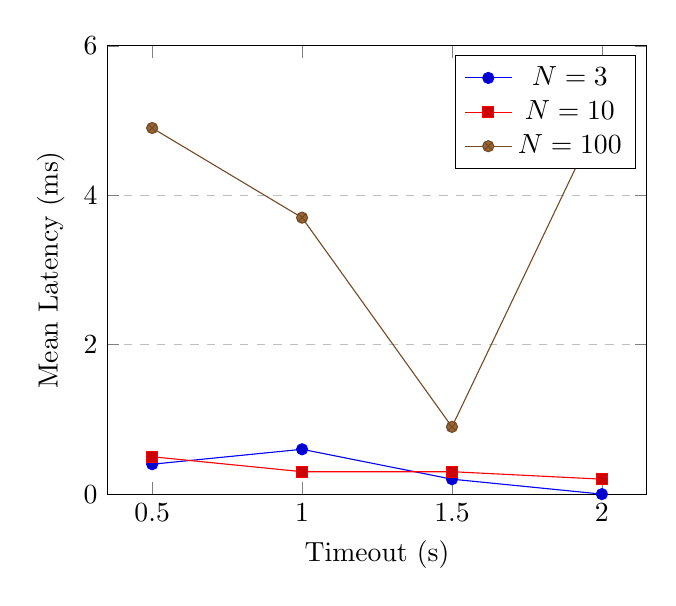
\begin{tikzpicture}
        \begin{axis}[
            xlabel={Timeout (s)},
            ylabel={Mean Latency (ms)},
            xtick=data,
            symbolic x coords={0.5, 1, 1.5, 2},
            ymin=0, ymax=6,
            ymajorgrids=true,
            grid style=dashed
        ]
        \addplot coordinates {(0.5, 0.4) (1, 0.6) (1.5, 0.2) (2, 0.0)};
        \addlegendentry{$N = 3$}
        \addplot coordinates {(0.5, 0.5) (1, 0.3) (1.5, 0.3) (2, 0.2)};
        \addlegendentry{$N = 10$}
        \addplot coordinates {(0.5, 4.9) (1, 3.7) (1.5, 0.9) (2, 5.1)};
        \addlegendentry{$N = 100$}
        \end{axis}
    \end{tikzpicture}
    \caption{Mean latency comparison for $\alpha = 0$}
\end{subfigure}%
\begin{subfigure}{.55\textwidth}
    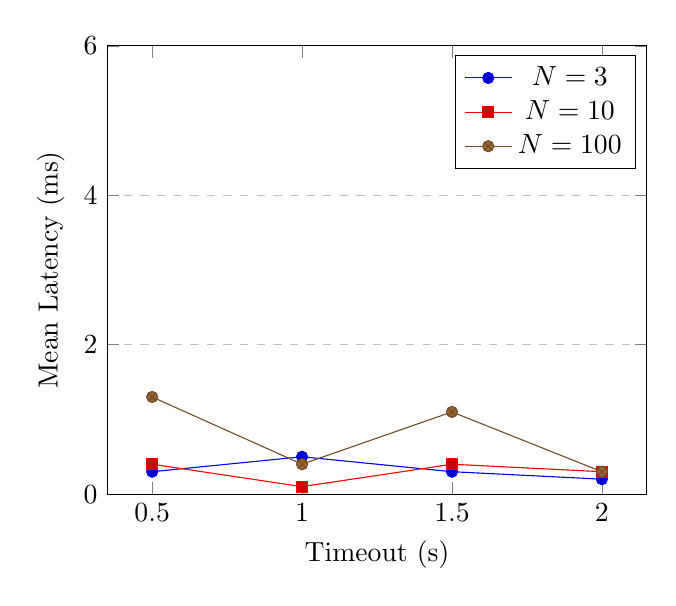
\begin{tikzpicture}
        \begin{axis}[
            xlabel={Timeout (s)},
            ylabel={Mean Latency (ms)},
            xtick=data,
            symbolic x coords={0.5, 1, 1.5, 2},
            ymin=0, ymax=6,
            ymajorgrids=true,
            grid style=dashed
        ]
        \addplot coordinates {(0.5, 0.3) (1, 0.5) (1.5, 0.3) (2, 0.2)};
        \addlegendentry{$N = 3$}
        \addplot coordinates {(0.5, 0.4) (1, 0.1) (1.5, 0.4) (2, 0.3)};
        \addlegendentry{$N = 10$}
        \addplot coordinates {(0.5, 1.3) (1, 0.4) (1.5, 1.1) (2, 0.3)};
        \addlegendentry{$N = 100$}
        \end{axis}
    \end{tikzpicture}
    \caption{Mean latency comparison for $\alpha = 0.1$}
\end{subfigure}
\begin{subfigure}{.55\textwidth}
    \vspace{1cm}
    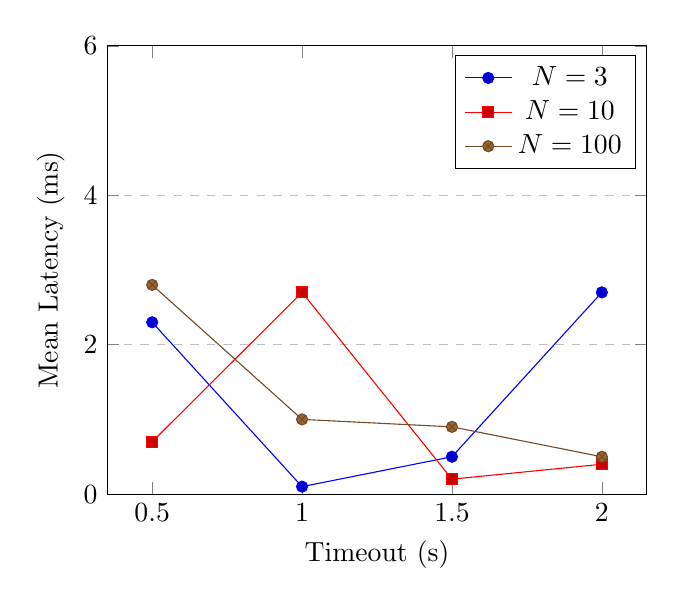
\begin{tikzpicture}
        \begin{axis}[
            xlabel={Timeout (s)},
            ylabel={Mean Latency (ms)},
            xtick=data,
            symbolic x coords={0.5, 1, 1.5, 2},
            ymin=0, ymax=6,
            ymajorgrids=true,
            grid style=dashed
        ]
        \addplot coordinates {(0.5, 2.3) (1, 0.1) (1.5, 0.5) (2, 2.7)};
        \addlegendentry{$N = 3$}
        \addplot coordinates {(0.5, 0.7) (1, 2.7) (1.5, 0.2) (2, 0.4)};
        \addlegendentry{$N = 10$}
        \addplot coordinates {(0.5, 2.8) (1, 1.0) (1.5, 0.9) (2, 0.5)};
        \addlegendentry{$N = 100$}
        \end{axis}
    \end{tikzpicture}
    \caption{Mean latency comparison for $\alpha = 1$}
\end{subfigure}
\caption{Mean latency comparison for fixed number of processes and alpha values}
\end{figure}

We can see here that the latency increases as the number of processes grows. This is due to the required quorum size needed to reach consensus. However, while having fewer processes can be faster, it is hardly scalable for more general use cases where a high number of requests may occur. With too few processes, the system risks overloading. Furthermore, with more processes, and given that at least
$ \frac{N}{2} + 1$ correct processes are required, the system can tolerate a higher number of failures.

\newpage

\subsection{Results for the probability of failure}
Let's now analyze the results for fixed numbers of processes $N$ and timeout $t_{le}$, with different probabilities of failure $\alpha$.

\begin{figure}[h!]
    \begin{subfigure}{0.55\textwidth}
    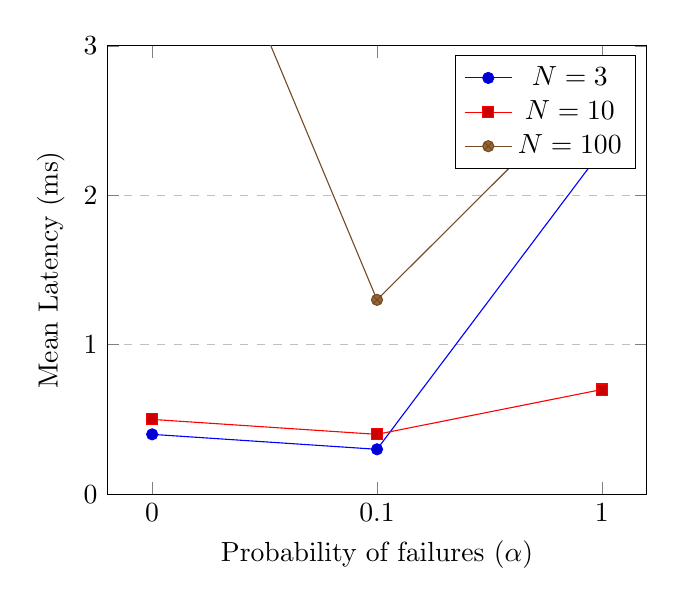
\begin{tikzpicture}
        \begin{axis}[
            xlabel={Probability of failures ($\alpha$)},
            ylabel={Mean Latency (ms)},
            xtick=data,
            symbolic x coords={0, 0.1, 1},
            ymin=0, ymax=3,
            ymajorgrids=true,
            grid style=dashed
        ]
        \addplot coordinates {(0, 0.4) (0.1, 0.3) (1, 2.3)};
        \addlegendentry{$N = 3$}
        \addplot coordinates {(0, 0.5) (0.1, 0.4) (1, 0.7)};
        \addlegendentry{$N = 10$}
        \addplot coordinates {(0, 4.9) (0.1, 1.3) (1, 2.8)};
        \addlegendentry{$N=100$}
        \end{axis}
    \end{tikzpicture}
\caption{Mean latency for $t_{le} = 0.5s$}

\end{subfigure}%
\begin{subfigure}{.55\textwidth}
    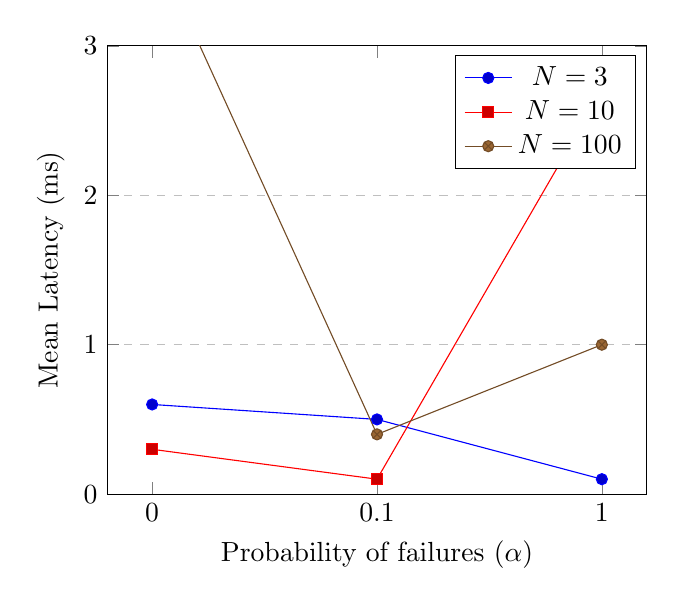
\begin{tikzpicture}
        \begin{axis}[
            xlabel={Probability of failures ($\alpha$)},
            ylabel={Mean Latency (ms)},
            xtick=data,
            symbolic x coords={0, 0.1, 1},
            ymin=0, ymax=3,
            ymajorgrids=true,
            grid style=dashed
        ]
        \addplot coordinates {(0, 0.6) (0.1, 0.5) (1, 0.1)};
        \addlegendentry{$N = 3$}
        \addplot coordinates {(0, 0.3) (0.1, 0.1) (1, 2.7)};
        \addlegendentry{$N = 10$}
        \addplot coordinates {(0, 3.7) (0.1, 0.4) (1, 1.0)};
        \addlegendentry{$N=100$}
        \end{axis}
    \end{tikzpicture}

\caption{Mean latency for $t_{le} = 1s$}
\end{subfigure}
\begin{subfigure}{.55\textwidth}
    \vspace{1cm}
    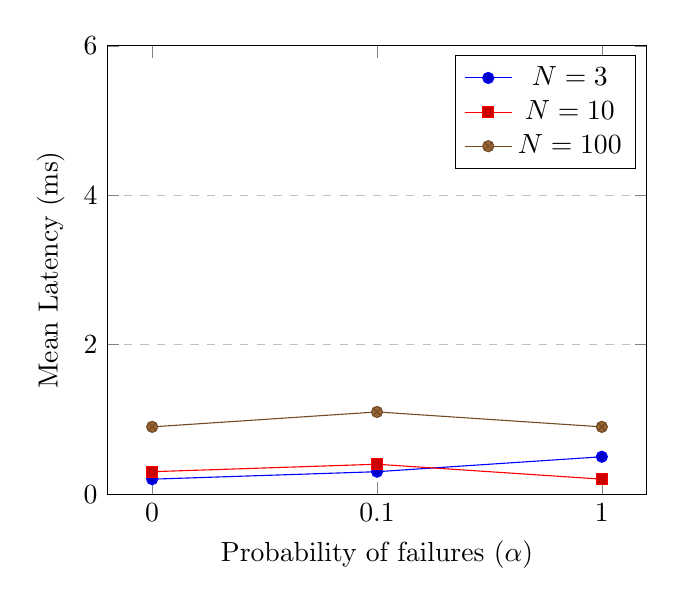
\begin{tikzpicture}
        \begin{axis}[
            xlabel={Probability of failures ($\alpha$)},
            ylabel={Mean Latency (ms)},
            xtick=data,
            symbolic x coords={0, 0.1, 1},
            ymin=0, ymax=6,
            ymajorgrids=true,
            grid style=dashed
        ]

        \addplot coordinates {(0, 0.2) (0.1, 0.3) (1, 0.5)};
        \addlegendentry{$N = 3$}
        \addplot coordinates {(0, 0.3) (0.1, 0.4) (1, 0.2)};
        \addlegendentry{$N = 10$}
        \addplot coordinates {(0, 0.9) (0.1, 1.1) (1, 0.9)};
        \addlegendentry{$N = 100$}

        \end{axis}
    \end{tikzpicture}
\caption{Mean latency for $t_{le} = 1.5s$}
\end{subfigure}
\begin{subfigure}{.55\textwidth}
    \vspace{1cm}
    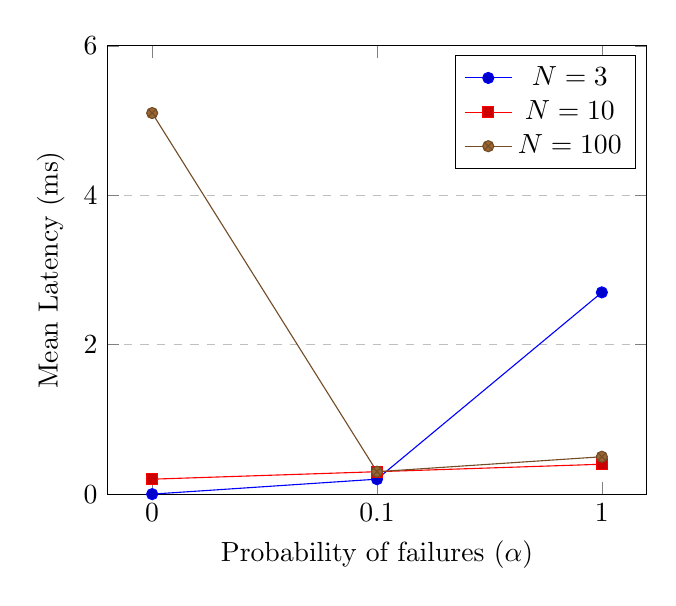
\begin{tikzpicture}
        \begin{axis}[
            xlabel={Probability of failures ($\alpha$)},
            ylabel={Mean Latency (ms)},
            xtick=data,
            symbolic x coords={0, 0.1, 1},
            ymin=0, ymax=6,
            ymajorgrids=true,
            grid style=dashed
        ]

        \addplot coordinates {(0, 0.0) (0.1, 0.2) (1, 2.7)};
        \addlegendentry{$N = 3$}
        \addplot coordinates {(0, 0.2) (0.1, 0.3) (1, 0.4)};
        \addlegendentry{$N = 10$}
        \addplot coordinates {(0, 5.1) (0.1, 0.3) (1, 0.5)};
        \addlegendentry{$N = 100$}

        \end{axis}
    \end{tikzpicture}
\caption{Mean latency for $t_{le} = 2s$}
\end{subfigure}
\caption{Mean latency comparison for fixed number of processes and alpha values}
\end{figure}

We can see in this part that the latency increases as the probability of failure
grows. This is due to the fact that the processes are more likely to fail, so they can't respond to requests and thus in order to reach a consensus, the process need to call all of the correct processes ($\frac{N}{2} + 1$).
\end{document}

